\section{Modelos}\label{sec:models}

Esta sección interpreta los modelos ajustados. Se distingue entre la estructura aprendida, es decir, reglas, coeficientes o funciones, y la evidencia de rendimiento ya presentada. La comparación se apoya en los mismos casos locales para mostrar qué explica cada familia y dónde coinciden o discrepan sus lecturas.

\subsection{Modelo lógico: reglas y probabilidades}

El árbol seleccionado puede leerse como una lista finita de reglas, la Figura~\ref{fig:tree} muestra su estructura. La configuración elegida en las cinco particiones externas fue profundidad máxima 3 y un mínimo de 500 registros por hoja, con umbral 0,25; el modelo resultante tiene profundidad efectiva 3, ocho hojas y quince nodos, y emplea tres variables.

\begin{figure}[H]
	\centering
	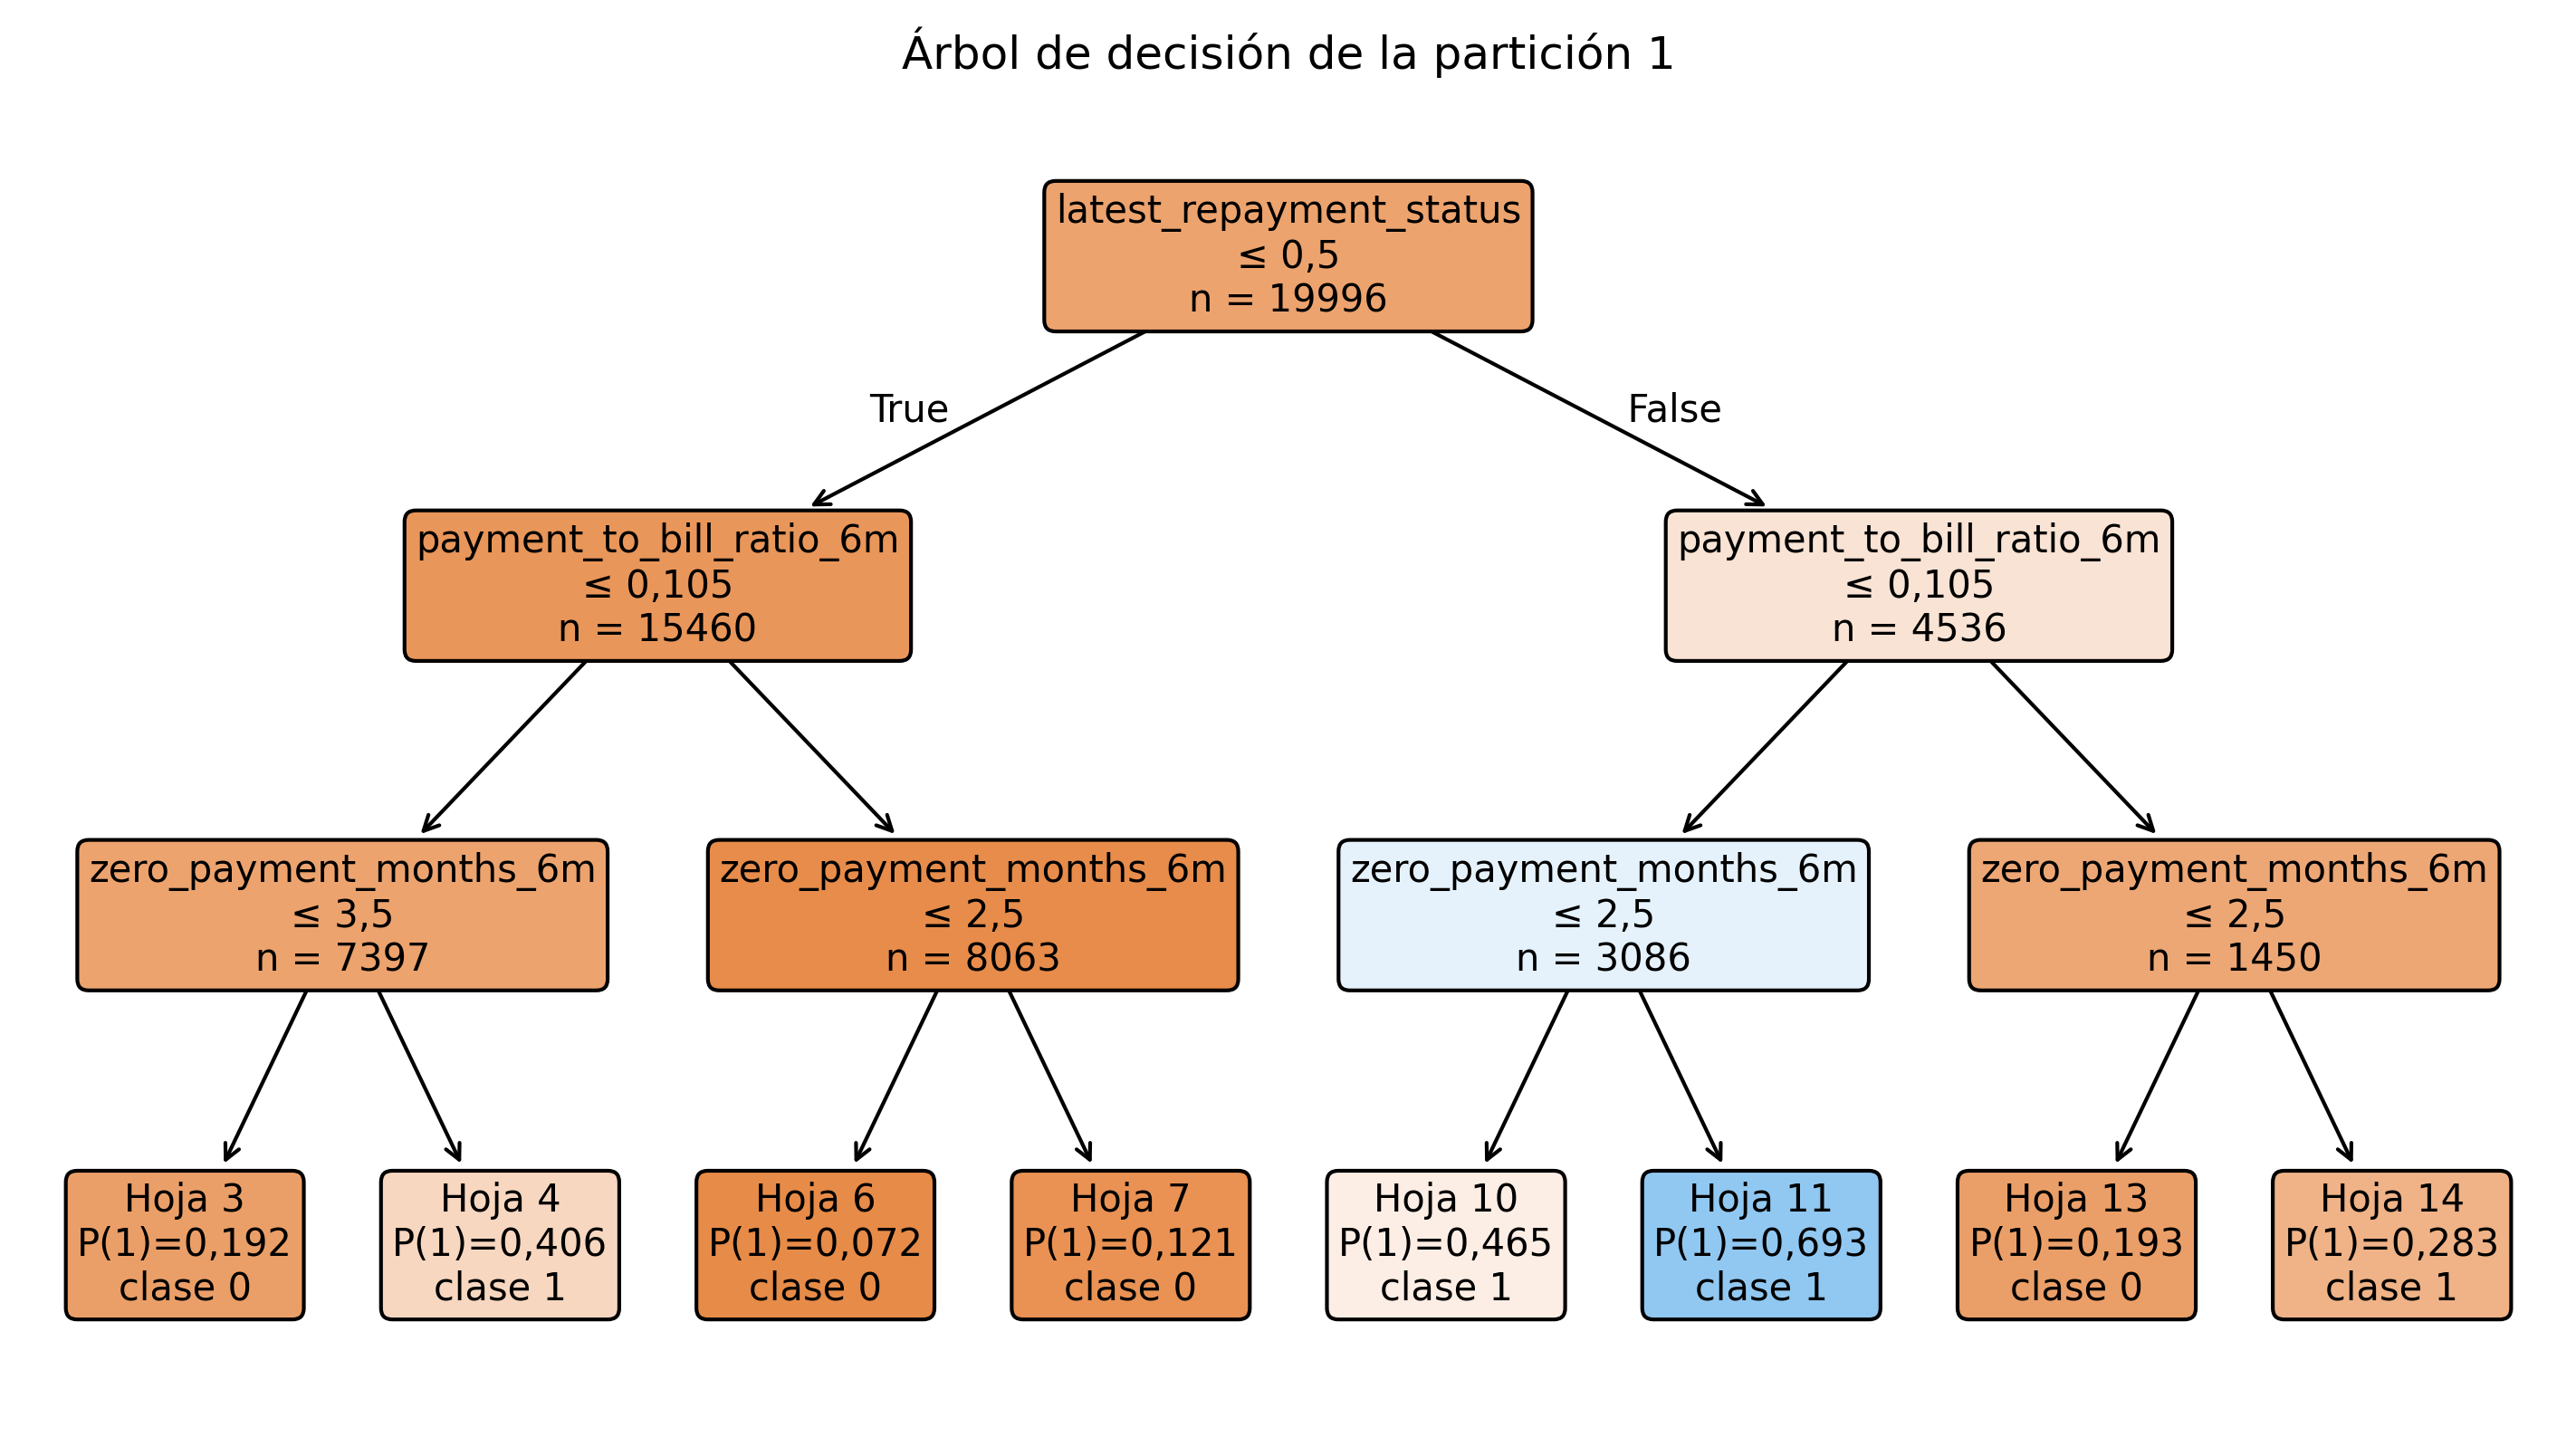
\includegraphics[width=\textwidth]{images/phase2_tree_names.png}
	\caption{Árbol de decisión de la partición 1. Cada nodo interno muestra la condición y el número de registros; cada hoja, la probabilidad estimada $P(1)$ y la clase asignada con el umbral 0,25.}
	\label{fig:tree}
\end{figure}

La raíz divide los registros según \var{latest_repayment_status}: $\le 0{,}5$ frente a $> 0{,}5$. El estado de pago más reciente es la primera distinción del modelo. La segunda división, repetida en ambas ramas, es \var{payment_to_bill_ratio_6m} $\le 0{,}105$, y el tercer nivel recurre a \var{zero_payment_months_6m} con umbrales $2{,}5$ o $3{,}5$. Las probabilidades de las hojas van de 0,0720 (hoja 6) a 0,6932 (hoja 11), de modo que el árbol no solo ordena los casos, sino que también expresa intensidades de riesgo muy distintas. La rama \var{latest_repayment_status} $\le 0{,}5$ contiene las hojas 3, 6 y 7, con probabilidades inferiores a 0,20, mientras que la hoja 4 alcanza 0,4062; la rama \var{latest_repayment_status} $> 0{,}5$ concentra tres de las cuatro hojas positivas (10, 11 y 14). Dentro de la rama de bajo \var{latest_repayment_status} y bajo \var{payment_to_bill_ratio_6m}, superar \var{zero_payment_months_6m} $= 3{,}5$ eleva la probabilidad de 0,1920 a 0,4062, más del doble. Con umbral 0,5 solo la hoja 11 predeciría la clase 1; al bajarlo a 0,25 se añaden las hojas 4, 10 y 14, la sensibilidad pasa del 14,31\,\% al 48,90\,\% y la precisión cae de 0,6812 a 0,4805. El comportamiento operativo del árbol depende, por tanto, de una decisión externa al ajuste.

La importancia Gini de la partición 1 es 57,25\,\% para \var{latest_repayment_status}, 29,71\,\% para \var{payment_to_bill_ratio_6m} y 13,05\,\% para \var{zero_payment_months_6m}; las otras doce variables no se usan. Esa concentración explica la legibilidad del modelo y también su límite, ya que tres variables resumen el riesgo y el resto de la información queda fuera. Las probabilidades de las hojas son frecuencias de entrenamiento, no probabilidades calibradas, es decir, que una hoja con 0,4646 se clasifique como positiva depende del umbral escogido (0,25 en nuestro caso).

La estructura se repite entre particiones, ya que los cinco árboles comparten la raíz \var{latest_repayment_status} $\le 0{,}5$ y la división \var{payment_to_bill_ratio_6m} $\le 0{,}105$ en ambas ramas. El tercer nivel es menos estable, con \var{zero_payment_months_6m} en cuatro modelos, \var{delayed_months_6m} en tres, \var{age} en dos, y \var{utilization_sep} y \var{credit_limit} en uno cada uno, con umbrales variables. La importancia media confirma ese patrón, con $0{,}5697 \pm 0{,}0066$ para \var{latest_repayment_status}, $0{,}3111 \pm 0{,}0232$ para \var{payment_to_bill_ratio_6m}, $0{,}0757 \pm 0{,}0531$ para \var{zero_payment_months_6m} y $0{,}0390 \pm 0{,}0358$ para \var{delayed_months_6m}. Cabe concluir que los dos primeros niveles son estables, mientras que las reglas terminales y sus probabilidades deben interpretarse con cautela.

\subsection{Coeficientes y odds ratios de la regresión logística}

La regresión logística supone que el logaritmo de las odds de dificultad de pago es una función lineal de los predictores transformados,
\[
\log\frac{P(Y=1\mid \mathbf{x})}{1-P(Y=1\mid \mathbf{x})}
= \beta_0 + \sum_{j=1}^{p}\beta_j z_j,
\]
donde $z_j$ representa una variable numérica estandarizada o una columna indicadora del one-hot. Cada $\beta_j$ cuantifica el cambio en log-odds asociado a una unidad de $z_j$ mientras el resto se mantiene fijo. Es una asociación condicional del modelo, no un efecto causal. La exponenciación da la odds ratio (OR), $\mathrm{OR}_j=e^{\beta_j}$, que expresa cuánto se multiplican las odds, no la probabilidad.

Las variables categóricas se codificaron con one-hot y la primera categoría como referencia, de modo que sus coeficientes se interpretan frente a ella. En la partición~1 las referencias son \var{female}, \var{graduate_school}, \var{married} y plan \var{no}. El término independiente, $-1{,}6022$, es el log-odds del perfil de referencia con todas las numéricas en su media, ya que están estandarizadas, y corresponde a una probabilidad de $16{,}77$\,\%. La tabla~\ref{tab:logistic-coefficients} recoge los ocho coeficientes principales de esa partición.

\begin{table}[H]
\centering
\footnotesize
\setlength{\tabcolsep}{6pt}
\begin{tabularx}{\textwidth}{@{}lrrX@{}}
\toprule
Entrada & Coeficiente & OR & Contraste \\
\midrule
\var{zero_payment_months_6m} & $0{,}5156$ & $1{,}6746$ & 1 DT $=1{,}7219$ meses \\
\var{repayment_assistance_plan_yes} & $0{,}4368$ & $1{,}5478$ & \var{yes} frente a \var{no} \\
\var{latest_repayment_status} & $0{,}4288$ & $1{,}5354$ & 1 DT  $=1{,}1215$ códigos \\
\var{utilization_sep} & $0{,}3841$ & $1{,}4683$ & 1 DT $=0{,}4050$ \\
\var{delayed_months_6m} & $0{,}2958$ & $1{,}3441$ & 1 DT $=1{,}5468$ meses \\
\var{total_payment_6m} & $-0{,}1682$ & $0{,}8500$ & 1 DT  $=58\,798{,}84$  \\
\var{maximum_repayment_delay_6m} & $-0{,}1216$ & $0{,}8900$ & 1 DT  $=1{,}0678$ meses\\
\var{sex_male} & $-0{,}0430$ & $0{,}9600$ & \var{male} frente a \var{female} \\
\bottomrule
\end{tabularx}
\caption{Coeficientes y odds ratios de la regresión logística en la partición~1. Las variables numéricas se expresan por una desviación típica (DT); las categóricas, frente a la categoría de referencia.}
\label{tab:logistic-coefficients}
\end{table}

Dos advertencias son necesarias para leer la tabla. Primero, los coeficientes de las numéricas se expresan por una desviación típica, no por una unidad original. Una OR de $1{,}6746$ en \var{zero_payment_months_6m} corresponde a $1{,}7219$ meses, y la de \var{utilization_sep}, $1{,}4683$, a $0{,}4050$ unidades de utilización. Segundo, una OR mayor que uno aumenta las odds, no la probabilidad, porque la conversión depende de la probabilidad de partida, de modo que multiplicar las odds por $1{,}5478$ no multiplica la probabilidad por esa cifra.

Los signos positivos principales corresponden a los meses sin pago, el plan de asistencia, el estado de devolución, la utilización y los meses con retraso, todos ellos se asocian con odds mayores. En sentido contrario, el total pagado, el retraso máximo y el sexo masculino presentan coeficientes negativos. El signo negativo del retraso máximo es condicional a los demás resúmenes de retraso, muy correlacionados entre sí; su correlación de Spearman con los meses con retraso es $0{,}982$. No implica que retrasarse proteja, sino que, una vez contabilizada la acumulación de meses, el máximo aporta información adicional en sentido opuesto. La lectura conjunta de variables correlacionadas exige cautela.

La penalización L1 fue seleccionada en las cinco particiones, con $C$ entre $0{,}1$ y $10$, y mantuvo entre 15 y 19 coeficientes no nulos de las 19 columnas transformadas. En la partición~1 anuló \var{education_other}, \var{education_unknown} y dos categorías de estado civil; un cero no prueba irrelevancia, pues depende de la penalización, de la colinealidad y de la frecuencia de la categoría. La estabilidad es razonable en los términos dominantes. El mismo conjunto de 19 entradas se repite en los cinco modelos, sin inversiones de signo, con magnitudes parecidas en los meses sin pago ($0{,}5051 \pm 0{,}0095$), el estado de devolución ($0{,}4151 \pm 0{,}0133$), la utilización ($0{,}3926 \pm 0{,}0120$) y el plan ($0{,}4520 \pm 0{,}0262$), mientras el total pagado se mantiene negativo ($-0{,}1692 \pm 0{,}0089$). Las categorías poco frecuentes alternan entre cero y no cero, por lo que su presencia concreta no debe interpretarse como un hallazgo estable. En conjunto, la logística ofrece una representación compacta y consistente en los términos dominantes, aunque su lectura exige recordar la escala estandarizada y la categoría de referencia.

\subsection{Funciones aditivas y formas aprendidas del EBM}

El EBM, ajustado sin interacciones, es un modelo aditivo generalizado en el que la puntuación de un registro se escribe como un valor independiente más la suma de quince funciones univariantes, una por predictor:
\[
\mathrm{logit}\, P(1 \mid \mathbf{x}) = \beta_0 + \sum_{j=1}^{15} f_j(x_j).
\]
En esta especificación, cada función depende de una sola variable y puede inspeccionarse por separado. La contribución $f_j(x_j)$ se expresa en log-odds, no una probabilidad ni un efecto causal, y solo se interpreta junto con las demás funciones. El valor independiente es $-1{,}6001$, de modo que un registro cuya suma de contribuciones sea cero tiene una probabilidad estimada del $16{,}80$ \%. Con quince funciones, el modelo es más expresivo que la regresión logística, pero sigue siendo aditivo y, por tanto, descomponible. Para un registro concreto, la predicción se reconstruye sumando el valor independiente y las quince contribuciones, lo que permite auditar por separado cada variable.

La tabla \ref{tab:ebm-importance} resume seis funciones seleccionadas de la partición 1. La importancia es la media del valor absoluto de la contribución y ordena las variables, pero no indica el signo ni la forma de la relación, que deben leerse en cada función. Una importancia alta puede combinar contribuciones de signo opuesto en distintos tramos, de ahí la necesidad de examinar la forma.

\begin{table}[H]
\centering
\small
\begin{tabularx}{\textwidth}{@{}l c X@{}}
\toprule
Variable & Importancia global & Lectura \\
\midrule
\var{payment_to_bill_ratio_6m} (R) & 0,3158 & Mayor peso; forma no monótona. \\
\var{latest_repayment_status} (S) & 0,2445 & Aumenta con los códigos de retraso, con mesetas. \\
\var{zero_payment_months_6m} (Z) & 0,2134 & Uno y dos meses, menor contribución que cero meses; desde tres, positiva. \\
\var{delayed_months_6m} & 0,1830 & Crece con la acumulación de retrasos. \\
\var{repayment_assistance_plan} & 0,1632 & \textit{yes} frente a \textit{no}: $+0{,}491$ log-odds. \\
\var{age} & 0,1349 & No lineal; extremos con menos respaldo. \\
\bottomrule
\end{tabularx}
\caption{Importancia global de seis funciones del EBM en la partición 1. La importancia es la media del valor absoluto de la contribución, en log-odds. La última columna resume la forma observada.}
\label{tab:ebm-importance}
\end{table}

La figura \ref{fig:ebm-shapes} muestra cuatro de estas funciones. El cociente pagos/facturas (R) es el de mayor importancia y el de forma menos regular. Su contribución es positiva en valores muy bajos, negativa en la región intermedia y de nuevo positiva en el extremo alto. Esa no monotonía sugiere que el cociente mezcla situaciones distintas; los valores altos pueden reflejar pagos extraordinarios o denominadores pequeños, por lo que no deben leerse como una señal unívoca de riesgo. El estado de pago reciente (S) y los meses con retraso \var{delayed_months_6m} aumentan en general con los códigos positivos y con la acumulación de retrasos, aunque presentan mesetas. En los meses sin pago (Z), uno y dos meses presentan una contribución menor que la de cero meses, mientras que desde tres la contribución es positiva y creciente. La edad sigue un patrón no lineal: mayor contribución en los jóvenes, negativa en parte de la edad adulta y creciente en el tramo superior, con menos respaldo en los extremos. La función del plan, que no aparece en la figura, asigna a \textit{yes} una contribución aproximadamente $0{,}491$ log-odds mayor que a \textit{no}.

\begin{figure}[H]
\centering
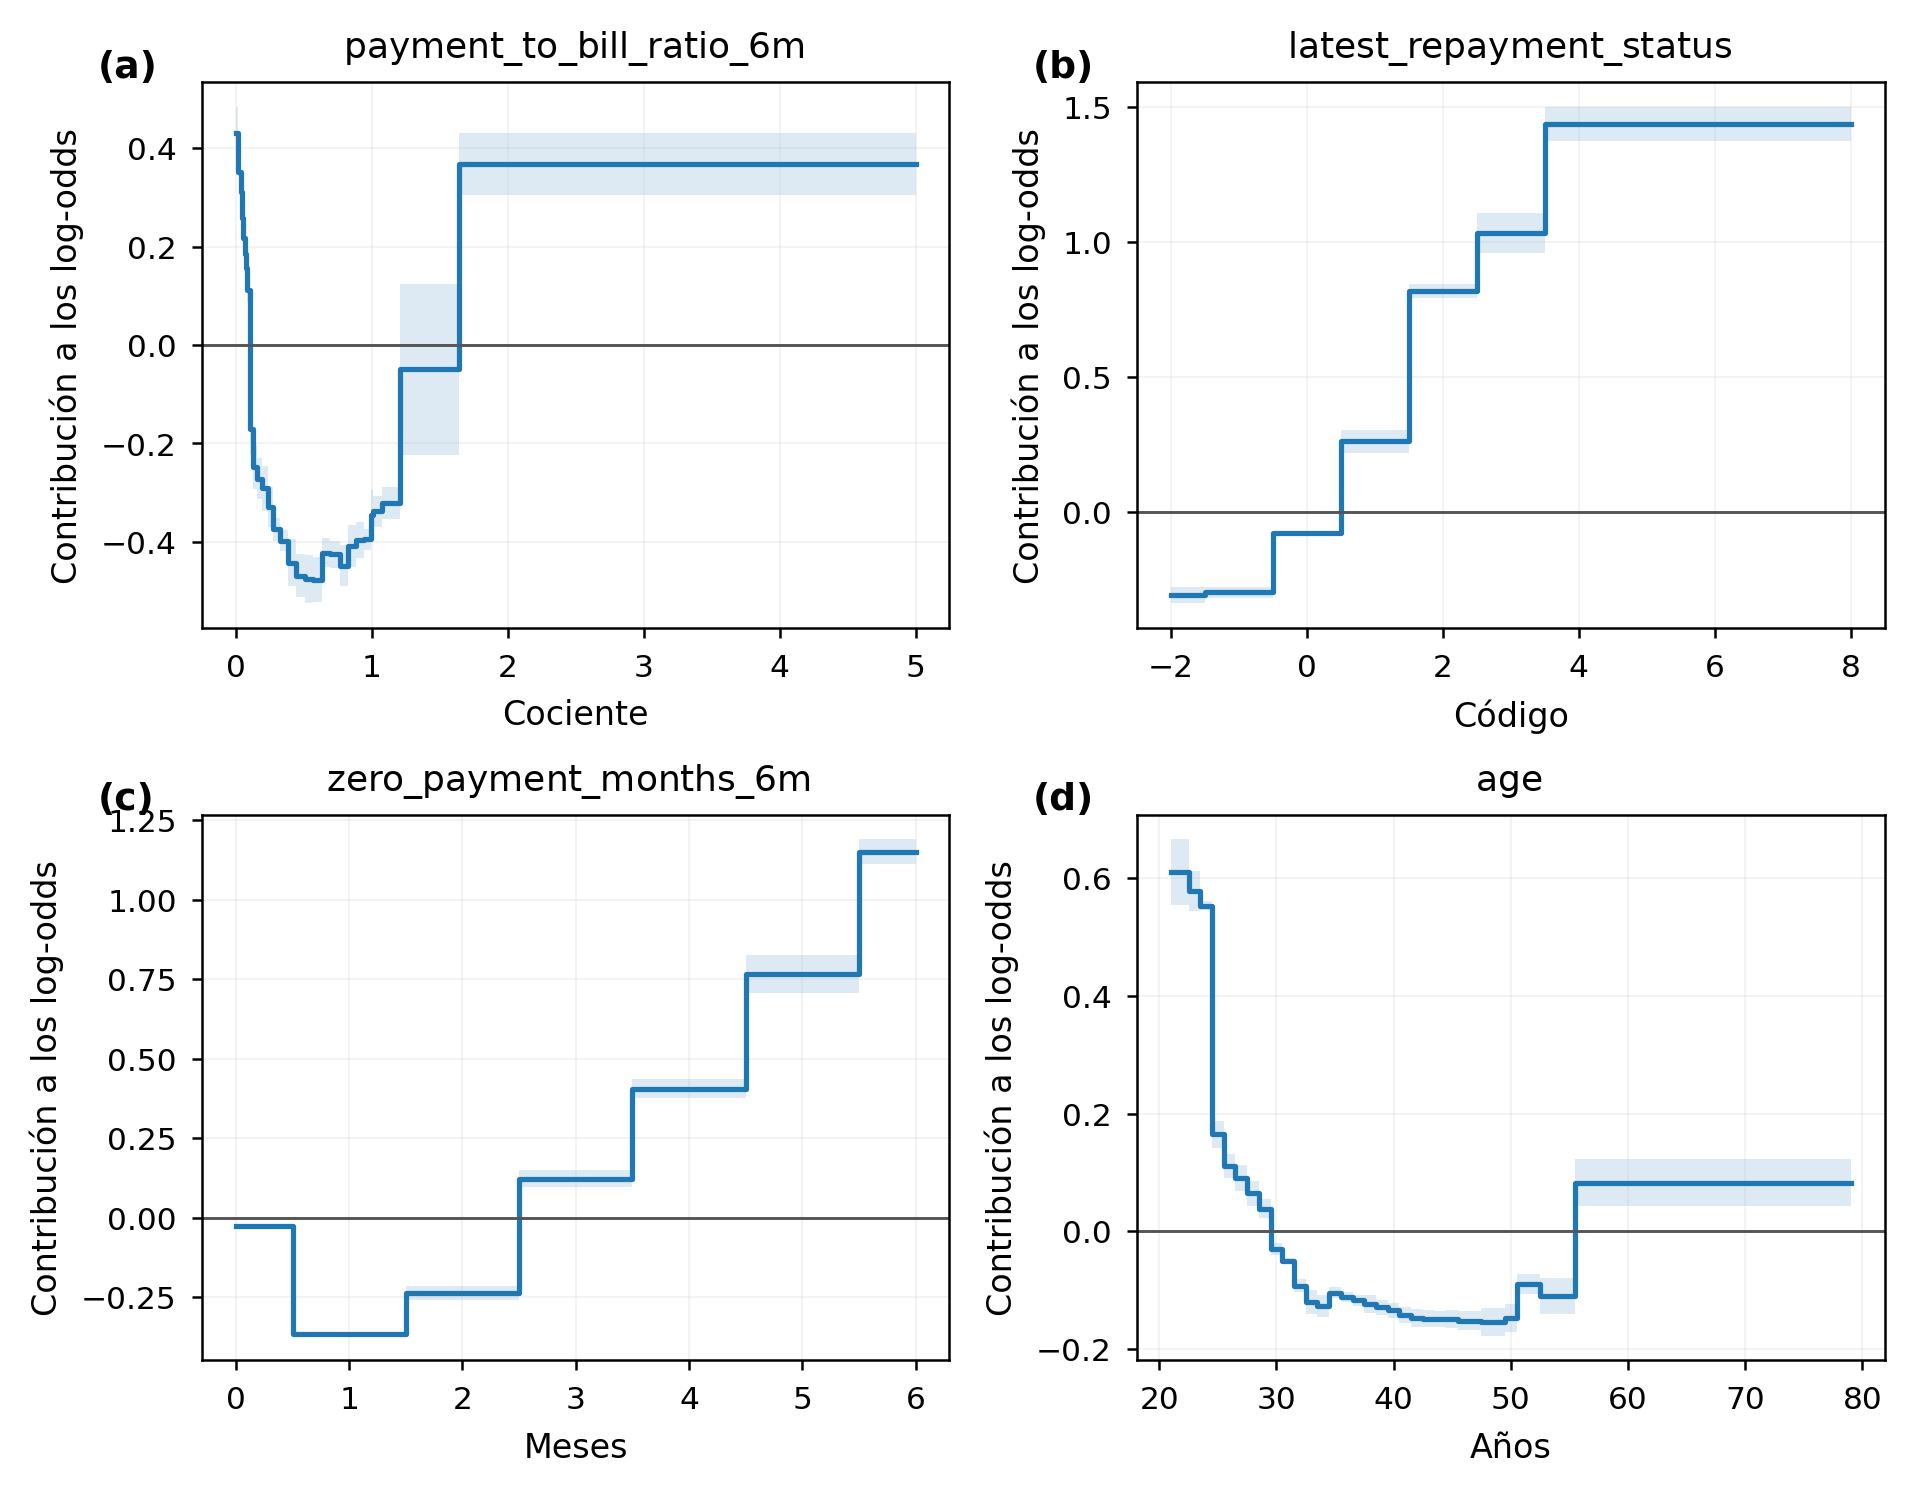
\includegraphics[width=0.7\textwidth]{images/phase2_ebm_shapes.png}
\caption{Cuatro funciones univariantes del EBM en la partición 1. En (a) se muestra el \var{payment_to_bill_ratio_6m}, en (b) el \var{latest_repayment_status}, en (c) \var{zero_payment_months_6m} y en (d) \var{age}. Las bandas representan la variabilidad entre las bolsas del modelo, no intervalos de confianza.}
\label{fig:ebm-shapes}
\end{figure}

En la figura \ref{fig:ebm-estability}, observamos que la estabilidad entre particiones es alta en lo esencial. R fue la función más importante en los cinco modelos, con una importancia media de $0{,}3072 \pm 0{,}0103$, después se repiten S, Z y \var{delayed_months_6m}, con cambios de orden. Las formas descritas reaparecen en las cinco particiones, la coincidencia de las formas es más informativa que el orden exacto de las importancias, y las discrepancias se concentran en los estados y recuentos altos y en las edades extremas, donde el respaldo de los datos es menor. En la partición 4 la contribución de S desciende del código 4 al 5, de modo que no puede afirmarse una monotonía universal. \var{maximum_repayment_delay_6m} presenta contribuciones positivas en algunos valores altos pese a su coeficiente logístico negativo. En conjunto, repetimos que estas formas son descripciones condicionales del modelo, no relaciones causales.


\begin{figure}[H]
	\centering
	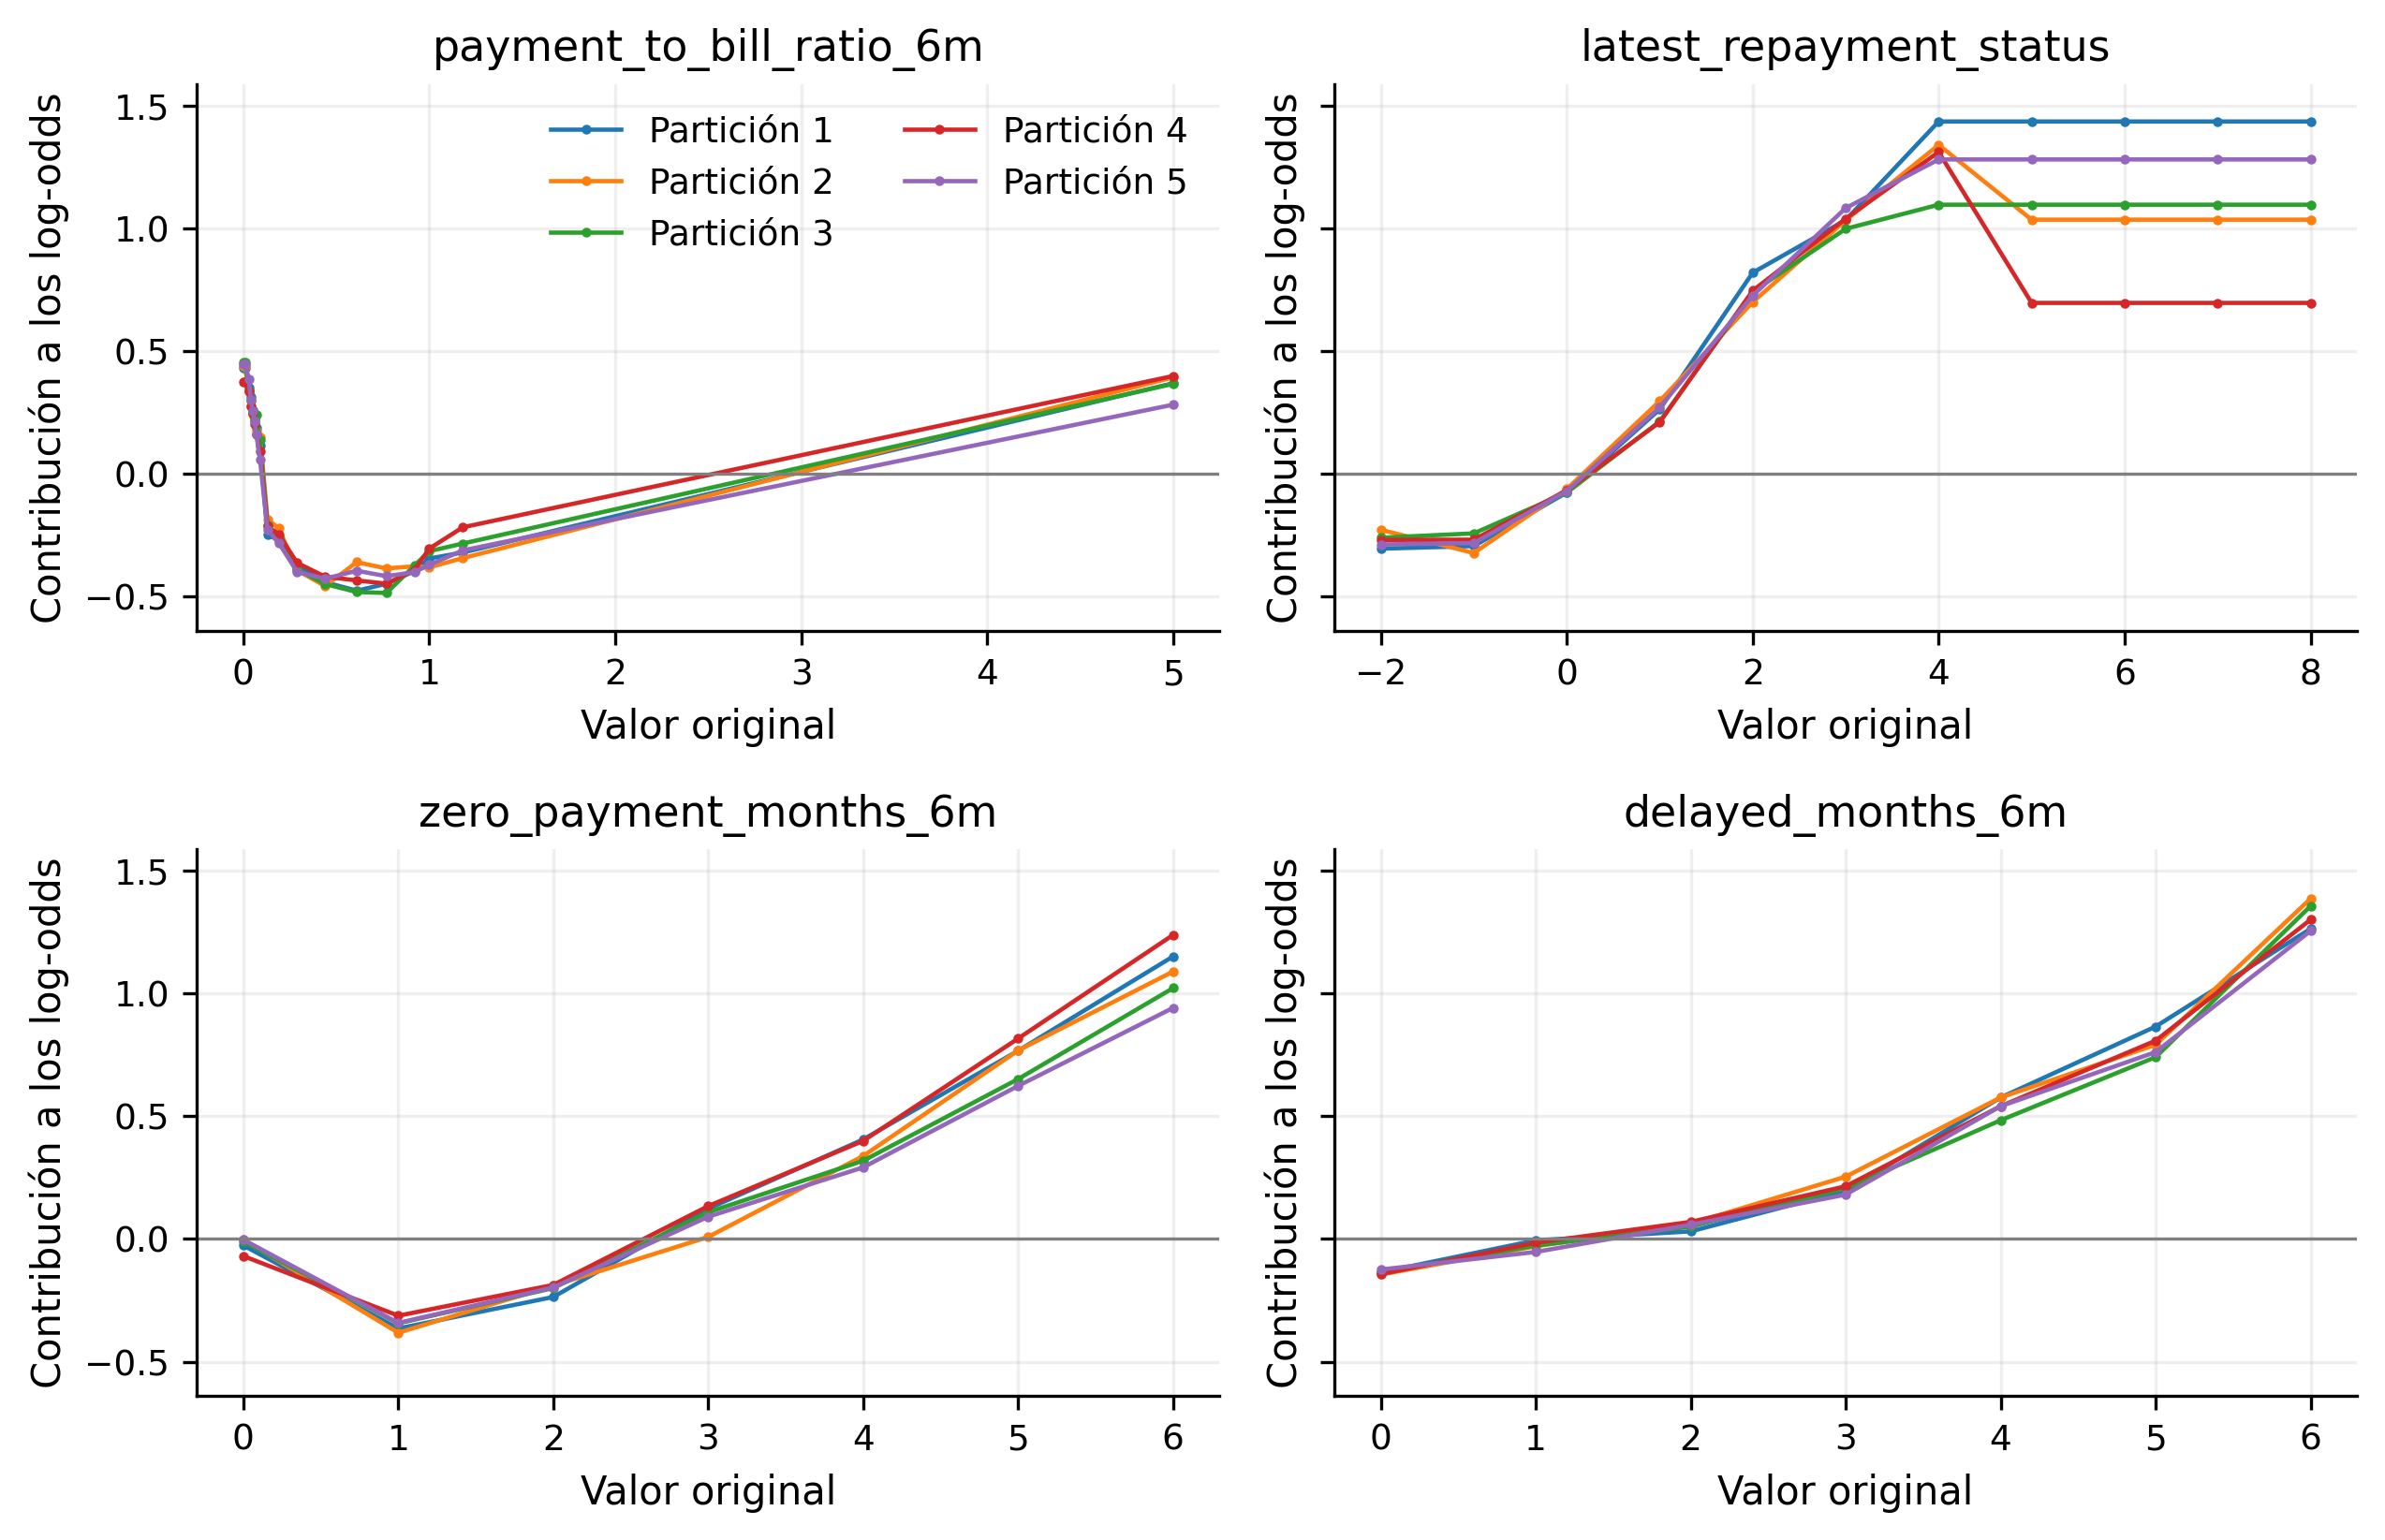
\includegraphics[width=0.7\textwidth]{images/phase2_ebm_stability.png}
	\caption{Estabilidad de cuatro funciones del EBM entre las cinco particiones. En (a) se muestra \var{payment_to_bill_ratio_6m}, en (b) \var{latest_repayment_status}, en (c) \var{zero_payment_months_6m} y en (d) \var{delayed_months_6m}. Cada color corresponde a una partición y la contribución se expresa en log-odds.}
	\label{fig:ebm-estability}
\end{figure}


\subsection{Explicaciones locales comparadas}

Para contrastar las explicaciones más allá de los resúmenes globales, se examinaron cuatro registros de la partición 1 con sus umbrales internos: $0{,}25$ para el árbol y la regresión logística, y $0{,}20$ para el EBM. La Tabla~\ref{tab:local-cases} recoge las probabilidades estimadas de la clase 1. Las cuatro probabilidades son inferiores a $0{,}5$, de modo que la decisión depende del umbral y no solo del orden entre modelos.


\begin{table}[H]
	\centering
	\small
	\caption{Cuatro casos locales de la partición 1 comparados entre familias. Los umbrales internos son $0{,}25$ para árbol y logística y $0{,}20$ para EBM. $P(1)$ denota la probabilidad estimada de la clase 1.}
	\label{tab:local-cases}
	\begin{tabularx}{\textwidth}{@{}c c X c c c@{}}
		\toprule
		Caso & Clase real & Escenario & Árbol $P(1)$ & Logística $P(1)$ & EBM $P(1)$ \\
		\midrule
		1 & $0$ & Acuerdo correcto, clase 0 & $0{,}0720$ & $0{,}0444$ & $0{,}0582$ \\
		2 & $1$ & Acuerdo correcto, clase 1 & $0{,}4646$ & $0{,}3997$ & $0{,}2663$ \\
		3 & $0$ & Árbol y logística aciertan; EBM falso positivo & $0{,}1920$ & $0{,}1832$ & $0{,}2110$ \\
		4 & $1$ & Falso negativo compartido & $0{,}1208$ & $0{,}1539$ & $0{,}1364$ \\
		\bottomrule
	\end{tabularx}
\end{table}

El caso 1 (clase 0) es un acuerdo correcto con explicaciones distintas. El árbol llega a la hoja 6 (\var{latest_repayment_status} $\le 0{,}5$, \var{payment_to_bill_ratio_6m} $> 0{,}105$, \var{zero_payment_months_6m} $\le 2{,}5$), la logística subraya \var{latest_repayment_status}, \var{zero_payment_months_6m} y \var{total_payment_6m} con contribuciones negativas, y el EBM destaca \var{payment_to_bill_ratio_6m} y \var{latest_repayment_status}. El único que aparece en las tres lecturas es \var{latest_repayment_status}, y el árbol comparte \var{zero_payment_months_6m} con la logística y \var{payment_to_bill_ratio_6m} con el EBM.

El caso 3 (clase 0) es el único desacuerdo. El árbol ($0{,}1920$) y la logística ($0{,}1832$) quedan por debajo de su umbral y aciertan, mientras que el EBM asigna $0{,}2110$, supera su umbral en $1{,}10$ puntos porcentuales y produce un falso positivo. Entre las atribuciones principales, cada par comparte una variable distinta (\var{zero_payment_months_6m} entre árbol y logística, \var{payment_to_bill_ratio_6m} entre árbol y EBM y \var{utilization_sep} entre logística y EBM) y ninguna coincide en los tres.

Los casos 2 y 4 no añaden un contraste nuevo. El 2 repite el acuerdo con \var{zero_payment_months_6m} aunque en sentidos opuestos ($+0{,}229$ en la logística y $-0{,}236$ en el EBM), y el 4 es un falso negativo compartido. Destacamos que las atribuciones son descripciones locales del modelo, es decir, coincidir en la decisión no implica coincidir en la explicación, y discrepar puede depender solo del umbral.
